\section{Examples of In-Situ Computation}\label{sec:examples}

In the following we will look at some examples to get a feeling for the applications.
\subsection{Unit Conversions}\label{sec:units}
Reading documents containing units that one is not familiar with, can be an annoying task and
automatic unit conversion is thus a useful example for in-situ computation. 
In this section we will describe two use cases for automatic unit conversions, both of which
are already implemented using the JOBAD framework\ednote{UR@MK do we need a citation here?}.

Before starting to convert something, the user can highlight all quantity
expressions in a given document. This results in a document, as shown in
Figure~\ref{fig:highlight}. We further use this snippet as running example.

\begin{figure}
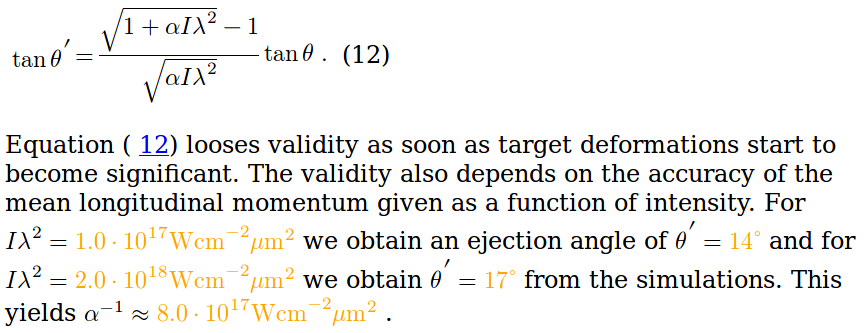
\includegraphics[scale=0.3]{screenshots/highlight.png}
\caption{An example of a document, where the quantity expressions are highlighted.}
\label{fig:highlight}
\end{figure}

In the first case, the user wants to convert a unit in just one expression to
an equivalent one, say watt to horsepower. For that, he can rightclick on this
particular expression and choose horsepower from the list of units that are
equivalent to watt. Figure~\ref{fig:convertone} demonstrates this and
Figure~\ref{fig:convertoneresult} displays the result of the computation. 

\begin{figure}
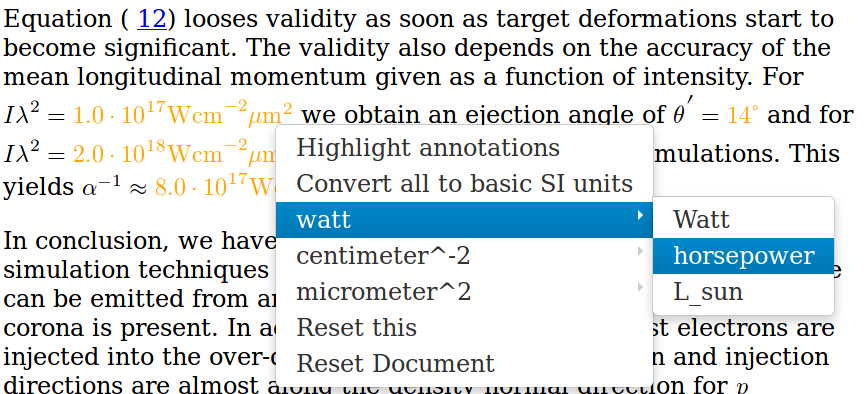
\includegraphics[scale=0.3]{screenshots/convertone.png}
\caption{The user can convert an expression, by choosing the desired
unit from a list of equivalent ones.}
\label{fig:convertone}
\end{figure}

\begin{figure}
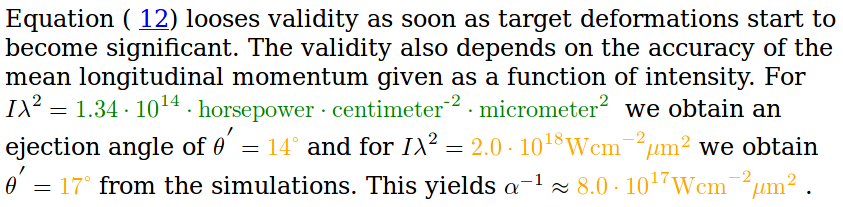
\includegraphics[scale=0.3]{screenshots/convertoneresult.png}
\caption{The result of the computation from Figure~\ref{fig:convertone}. 
The modified quantity expression is highlighted in orange.}
\label{fig:convertoneresult}
\end{figure}

The current example only allows local conversions, but of course the user also wants
to convert units document-wide -- ideally from one system of measurement to another. 
Figure~\ref{fig:si} shows the result of a prototypical implementation, which 
converts all units to irreducible SI base units. 
This could, for instance, be extended to automatically converts all quantity
expressions in a document from imperial to metric units and vice versa. 

\begin{figure}
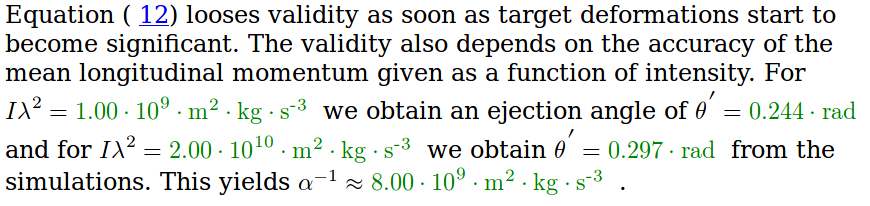
\includegraphics[scale=0.3]{screenshots/si.png}
\caption{All units have been converted to their corresponding SI base units for this example.}
\label{fig:si}
\end{figure}


\subsection{Equations}\label{sec:equations}

A common example of in-situ computation is the exploration of mathematical models that are
given as equations. In the simplest case, this can be equations like Einstein's
mass-energy equivalence (\ref{f:emc2}) -- which we will use as a running example -- and in
other cases, this can be complex models like van Roosbroeck's models for drift and
diffusion of electrons and holes in semiconductor devices~\cite{FarRotDoa:nmddm16}\footnote{We
  are currently studying this model, formalizing the inherent knowledge and augmenting
  (parts of) \cite{FarRotDoa:nmddm16} into an active document, see~\cite{KohKopMueTab:RCS} for
  first results. The methods reported on here will eventually be employed in this case
  study, which itself is beyond the scope of this deliverable report}, which comprises
partial differential equations, boundary conditions, and physical constants -- a much more
complex situation, but the possible interactions are essentially the same. 

So let us come back to our running example: The equation for mass-energy equivalence is
simple:

\begin{equation}\label{f:emc2}
  E=mc^2
\end{equation}

where $E$ is the energy, $m$ is the mass, and $c$ is the speed of light. It appears in
many documents, e.g. the Wikipedia article in Figure~\ref{fig:emc2-wikipedia}. In such a
document -- were it active -- a scholar or interested layman might be interested to see
what the energy equivalent of one gram of matter might be. Today a google query reveals a
custom-made answer at~\cite{Odenwald:q388}, but really our scholar would like to just right
click on the symbol $m$ in $\ref{f:emc2}$, instantiate it to $1g$ and have the document
\emph{simplify the changed expression} (in-situ computation) to give the answer.

Conversely, she might want to know how what mass it would take to drive e.g. from Erlangen
to Paris in a Tesla (which gets 6.25 km per kWh)\footnote{This is a natural and common
  question; see~\cite{RT:emc2} which computes the mileage a car would get out of a 1/16
  inch drop of water -- the value it comes up with is 96.000 miles.}. Here she would like
to just instantiate $E$ with $776 \times 6.25=4850$ kWh and the document \emph{solves the
  equation $4850=mc^2$ for $m$}.\ednote{MK: maybe do the computation and report the
  result} Of course, the result is so minuscule that she wants to have it changed to a
form she understand, e.g. the number of carbon atoms that weigh as much.

\begin{figure}\centering
  \begin{boxedquote}
    In physics, mass–energy equivalence states that anything having mass has an equivalent
    amount of energy and vice versa, with these fundamental quantities directly relating
    to one another by Albert Einstein's famous formula:

    \[E=mc^2\] 

    This formula states that the equivalent energy ($E$) can be calculated as the mass ($m$)
    multiplied by the speed of light ($c$ = about $3\times10^8 m/s$) squared.
  \end{boxedquote}
  \caption{From the Mass-Energy-Equivalence page at Wikipedia~\cite{WP:emc2}}
  \label{fig:emc2-wikipedia}
\end{figure}

Of course, the computations themselves in our example are rather simple, and can be
executed by any computer algebra system, and even complex examples like the van Roosbroeck
models alluded to above would tax modern systems exceedingly, indeed they are the kind
computations that are carried out and documented in Jupyter notebooks. 

The point here is that the envisioned in-situ computation service allows computation
without changing to another system and avoids errors (data entry errors and data
interpretation errors) induced by crossing system borders.

\subsection{Computation with Proofs}
\begin{itemize}
  \item calling automated theorem provers on a goal in a document
  \item extending the level of explanation by doing that on a subgoal or deepening the
    level of explanation. E.g. from ``obviously'' to a full proof.  
  \end{itemize}

\subsection{Hypothetical Computations Playing with Global/Local Values}\label{sec:hyp}
What would be paper look like if the speed of light were $88 mph$. 

\subsection{Updating Values to current or historical values}
spreadsheets (a well-understood form of active documents) can already do that. 
\begin{itemize}
\item global warming papers with newer models or data
\item Wolfram alpha: ``does it snow in hell?''
\end{itemize}




%%% Local Variables:
%%% mode: latex
%%% TeX-master: "report"
%%% End:

%  LocalWords:  sec:examples sec:units sec:equations f:emc2 Roosbroeck's Kopruckietal
%  LocalWords:  formalizing KohKopMueTab:RCS fig:emc2-wikipedia Odenwald:q388 emph
%  LocalWords:  RT:emc2 centering boxedquote WP:emc2 Roosbroeck Jupyter itemize sec:hyp
